\chapter{Progetto}
\label{chap:project}

\textit{Peer Network} supporta le aziende nella revisione e reingegnerizzazione dei processi aziendali, adottando un
approccio basato su \textbf{processi componibili}, un esempio è presente in \Cref{fig:composable-process}. Questo approccio
supera i limiti dei sistemi monolitici tradizionali, introducendo moduli autonomi, riutilizzabili e facilmente
combinabili, che garantiscono flessibilità e adattabilità di fronte ai cambiamenti operativi.

\begin{figure}
    \centering
    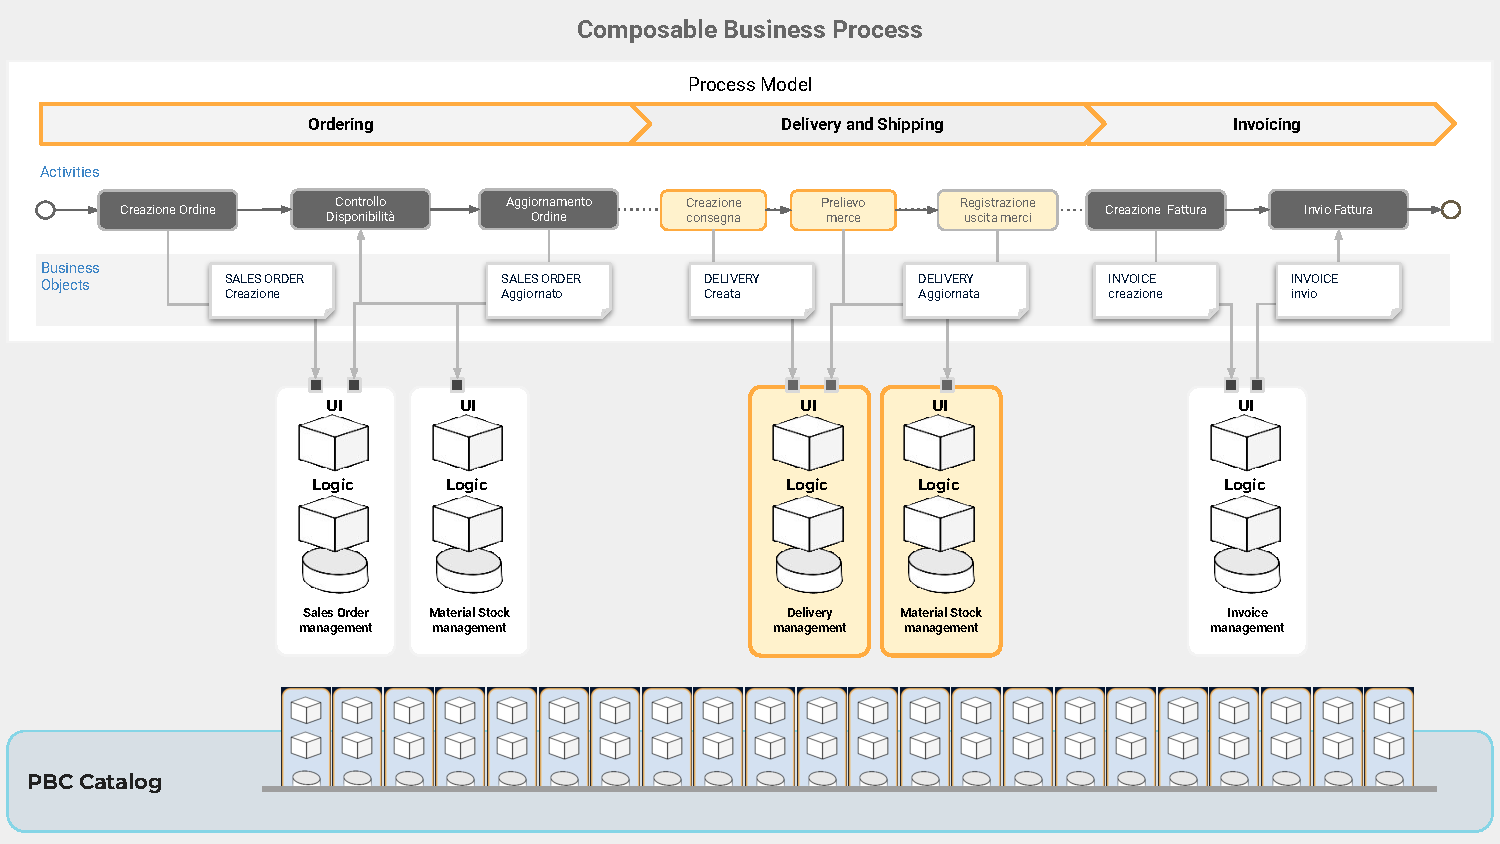
\includegraphics[width=\linewidth]{figures/composable_process.pdf}
    \caption{Struttura di un processo componibile}
    \label{fig:composable-process}
\end{figure}

La ridefinizione dei processi inizia identificando le attività da svolgere e gli \textbf{oggetti di business (BO)} coinvolti.
Gli oggetti di business rappresentano elementi chiave di un’organizzazione all’interno di un sistema informativo. Essi
riflettono entità reali, ad esempio cliente, prodotto, ordine, consegna, includendo ciascuno attributi specifici
(es. nell’ordine ci sono numero ordine, stato, riferimento ai prodotti). Questi oggetti, modellati in modo chiaro,
facilitano la gestione e l’integrazione dei processi aziendali, fungendo da base per la progettazione delle \ac{PBC}.

Per analizzare e modellare questi elementi, viene applicato il \textbf{Domain Driven Design}\cite{evans2004domain}, un metodo che consente di
suddividere il dominio aziendale in \textbf{Bounded Contexts} distinti. Ogni contesto rappresenta un sottoinsieme indipendente
e ben definito del dominio, facilitando la gestione e l’organizzazione dei processi.

All’interno di ciascun Bounded Context, gli oggetti di business vengono implementati come \textbf{\ac{PBC}}.
Queste unità modulari e riutilizzabili rappresentano specifiche entità aziendali che racchiudono in sé i dati e le azioni che
si possono compiere su di esse in un formato indipendente e facilmente integrabile. Come schematizzato nella \Cref{fig:pbc-struttura}
e nell’esempio in \Cref{fig:composable-process}, ciascuna \ac{PBC} descritta nelle ricerche di \textit{Gartner}\cite{natis2019innovation}\cite{burke2020top} include:

\begin{itemize}
    \item una \textbf{struttura dati} per rappresentare le informazioni associate alla \ac{PBC},
    \item un insieme di \textbf{API} di base per eseguire azioni sincrone sull'oggetto,
    \item un insieme di \textbf{eventi} di base per l'integrazione asincrona,
    \item una o più \textbf{interfacce utente} (opzionale).
\end{itemize}

\begin{figure}
    \centering
    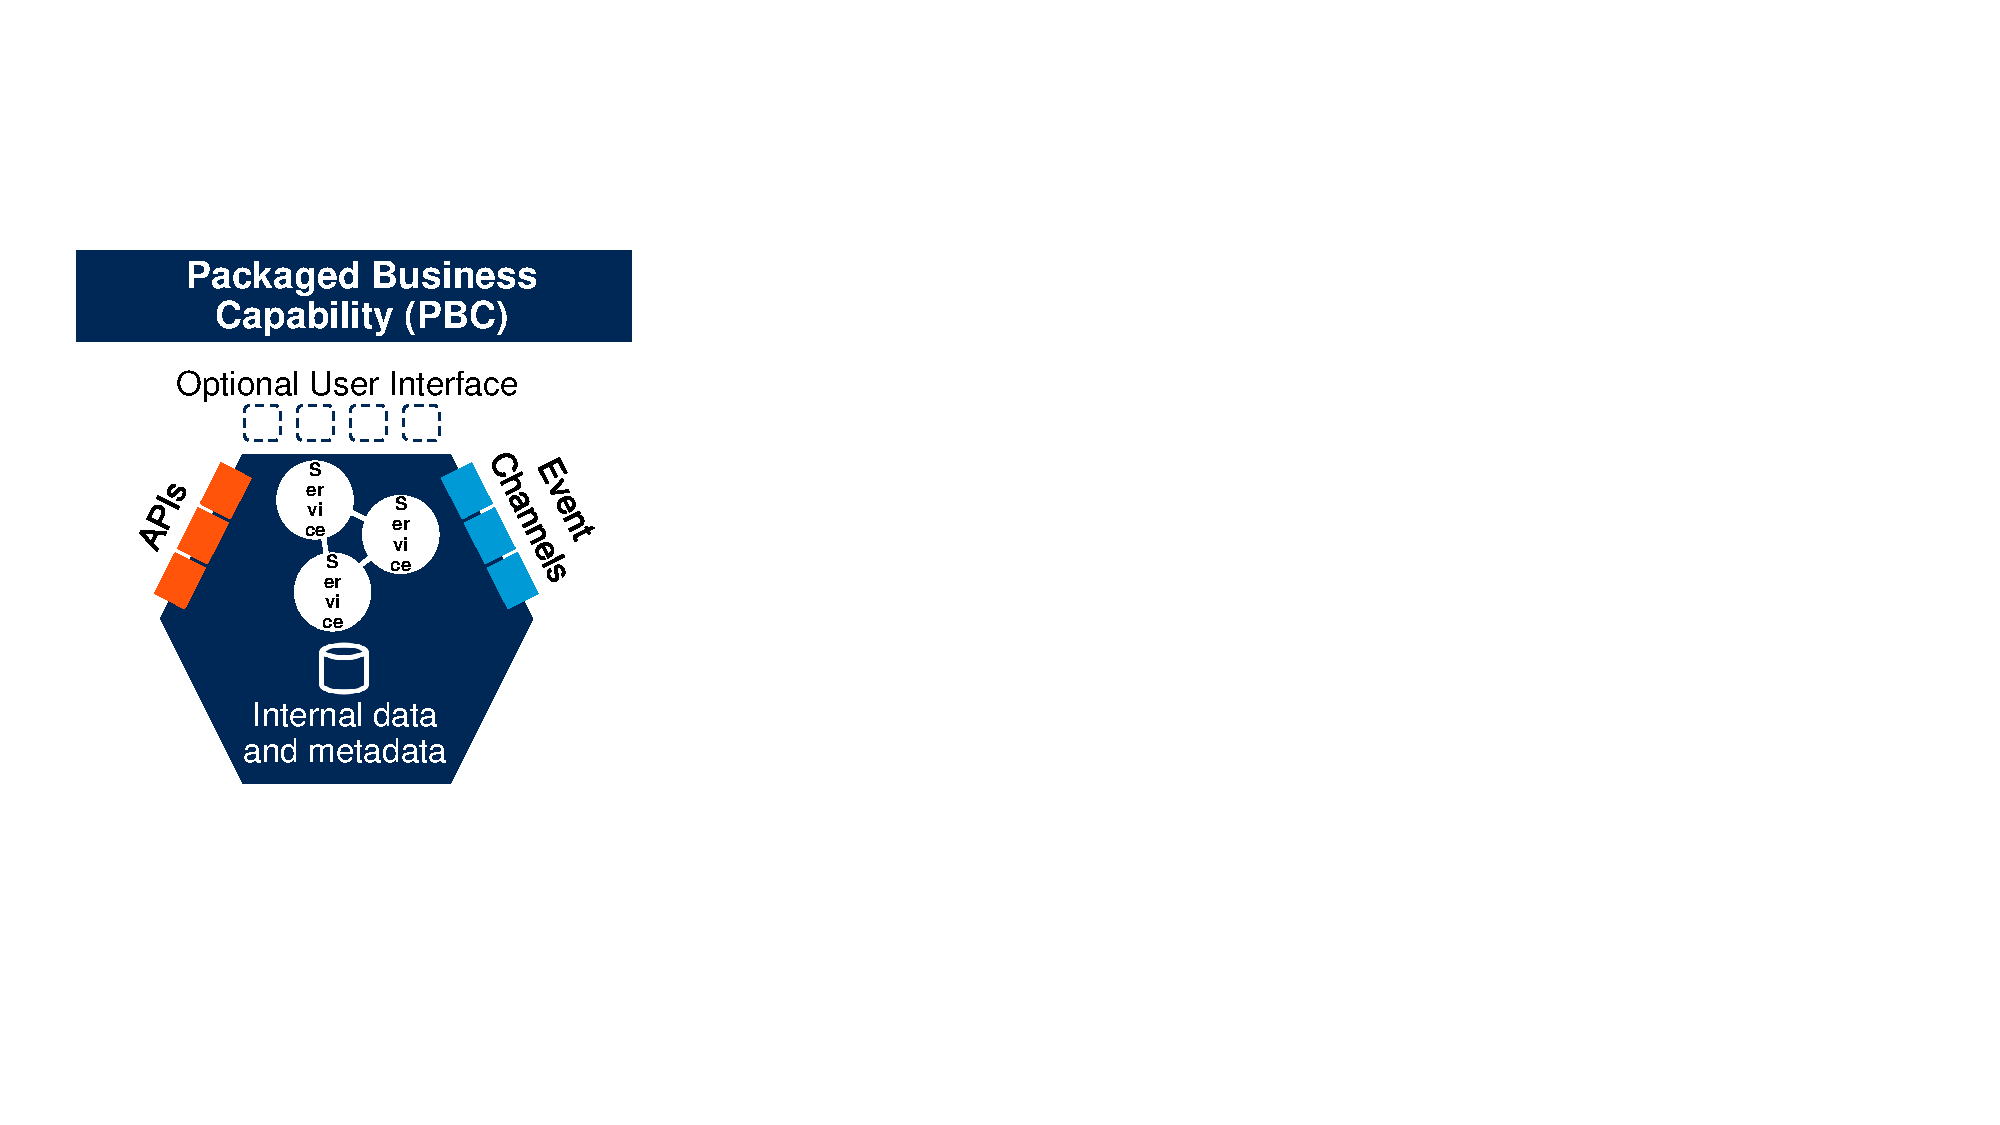
\includegraphics[scale=0.6]{figures/PBCstructure.pdf}
    \caption{Struttura \ac{PBC} secondo \textit{Gartner}}
    \label{fig:pbc-struttura}
\end{figure}

Questa struttura consente di progettare \textbf{applicazioni componibili}, assemblate combinando \ac{PBC} esistenti o sviluppandone di nuove.
Secondo \textit{Gartner}, tale approccio accelera il time-to-market, migliora l’adattabilità ai cambiamenti e garantisce soluzioni coerenti
con le esigenze operative dei clienti. Le applicazioni componibili sono progettate per richiamare dinamicamente i servizi dei
sistemi sottostanti, adottando un modello di integrazione process-centric, dove i processi di business guidano l’organizzazione
anziché i dati o le singole applicazioni. Questo tipo di applicazioni hanno una struttura che distingue chiaramente due livelli:

\begin{itemize}
    \item \textbf{frontend}, focalizzato sull’esperienza utente (UX) e costruito con interfacce intuitive,
    \item \textbf{backend}, dedicato alla logica applicativa, implementato tramite \ac{PBC} indipendenti.
\end{itemize}

Una delle caratteristiche distintive di \textit{Peer Network} è la capacità di trasferire su componenti di business, le \ac{PBC} appunto, le proprie
competenze di dominio e costruire con esse soluzioni componibili, invece di sviluppare software interamente personalizzati per ogni cliente.
Questo approccio è stato favorito dall’esperienza che l’azienda ha maturato in tanti anni di attività sulla piattaforma \ac{ERP} di
SAP\footnote{https://www.sap.com/italy/index.html}, che ha storicamente definito i principali standard internazionali nel settore.

Le soluzioni di \textit{Peer Network} semplificano il lavoro dei diversi attori di un processo di business, grazie a flussi operativi chiari e una
gestione meno complessa rispetto alle tradizionali piattaforme \ac{ERP}, come SAP. L'integrazione con la piattaforma \ac{ESI}, che funge anche da
repository per le \ac{PBC}, permette ai sistemi sviluppati di comunicare direttamente con gli \ac{ERP} aziendali. Questo processo non solo facilita
il recupero e l'elaborazione dei dati necessari, ma introduce anche una serie di funzionalità aggiuntive. Le informazioni così ottenute vengono
presentate attraverso interfacce grafiche progettate per ottimizzare usabilità ed efficienza operativa.

\section{Gestione Progetti}
\label{sec:pm}
Nel corso del tempo, nonostante gli sforzi per migliorare l’organizzazione e incrementare l’efficienza lavorativa, in \textit{Peer Network} sono
emerse difficoltà nel gestire contemporaneamente tutti i progetti. Questi ultimi si dividono in due principali categorie:

\begin{itemize}
    \item \textbf{progetti esterni}: soluzioni sviluppate per i clienti, denominate \ac{SBS},
    \item \textbf{progetti interni}, suddivisi ulteriormente in due tipologie:
        \begin{itemize}
            \item \textbf{ricerca e sviluppo}: attività principale è l'aggiornamento continuo delle \ac{PBC} per integrarle
            rapidamente nelle soluzioni destinate ai clienti e il conseguente miglioramento della piattaforma \ac{ESI};
            \item \textbf{software gestionale \ac{PAM}}: applicazione utilizzata internamente per il monitoraggio e la gestione del lavoro svolto dai dipendenti.
        \end{itemize}
\end{itemize}

Nel contesto di questa complessità operativa e dinamicità, i project manager e i dipendenti hanno individuato alcune problematiche generali.
La più evidente è la scarsità di personale rispetto al carico di lavoro, che porta gli sviluppatori a ricoprire più ruoli contemporaneamente,
sia all’interno dello stesso progetto sia su più progetti. Questo sovraccarico rende difficile per ciascuno svolgere al meglio i compiti assegnati.
Inoltre, i project manager, provenienti da un background tecnico, tendono ad adottare un approccio eccessivamente orientato agli aspetti tecnici,
trascurando l'analisi di dominio e la pianificazione strategica. Un ulteriore ostacolo è rappresentato dalla difficoltà nel delegare compiti: le
competenze sono concentrate in poche persone esperte e il coinvolgimento di risorse junior richiede tempo e sforzi per formazione e supervisione,
che spesso vengono percepiti come un rallentamento delle attività.

Per affrontare queste problematiche, l’azienda ha deciso di uniformare il più possibile la gestione dei progetti, adottando un approccio standardizzato
per l’intero ciclo di vita. Basandosi sui principi del \textbf{\ac{PMBOK}}\cite{project2021guide}, i project manager hanno quindi elaborato lo schema
del ciclo di vita ideale di un progetto in \textit{Peer Network}, riportato in \Cref{fig:fasi-progettuali}. Le future modifiche nella gestione dovranno
progressivamente allinearsi a questo modello.

Il ciclo di vita del progetto è stato suddiviso in tre fasi principali. La prima, denominata “Idea, Design, Economics”, prevede l’analisi iniziale di un
nuovo progetto, la progettazione, la definizione del budget e la stipula del contratto. La seconda fase “Progetto Software,” si concentra sull’analisi
approfondita dei requisiti, sulla pianificazione e sullo sviluppo, fino al rilascio del prodotto. La terza fase, “Supporto e Servizio,” riguarda l’assistenza
post-installazione e le attività di manutenzione correttiva per garantire il corretto funzionamento del sistema.

\begin{figure}
    \centering
    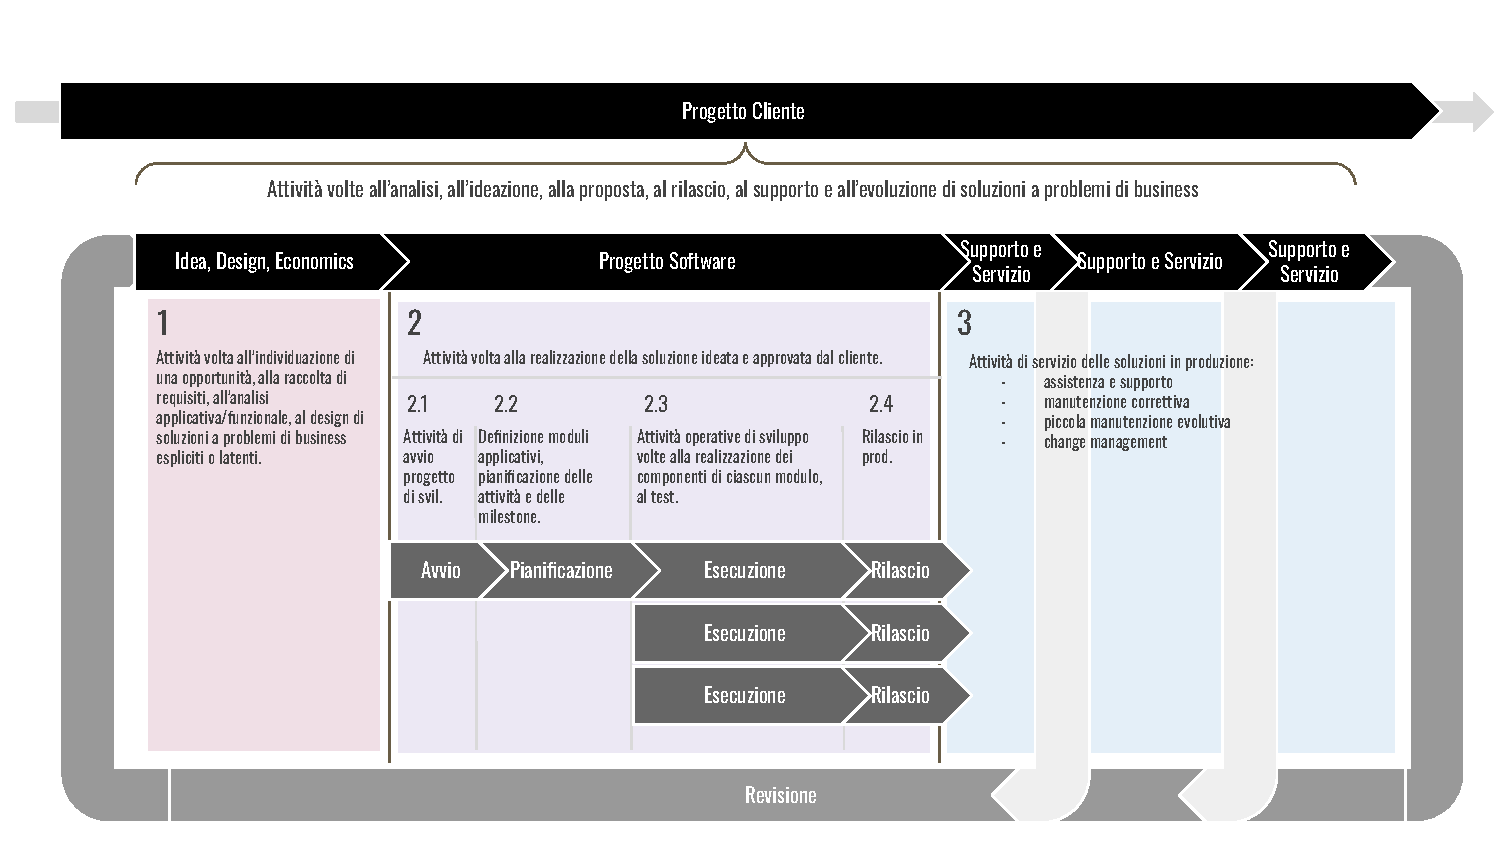
\includegraphics[width=\linewidth]{figures/FasiProgettualiPN.pdf}
    \caption{Ciclo di vita ideale per un progetto in \textit{Peer Network}}
    \label{fig:fasi-progettuali}
\end{figure}

Per raggiungere l'obiettivo di migliorare la gestione dei progetti, è innanzitutto fondamentale esaminare in dettaglio tutte le attività svolte nel novembre 2024,
identificando i problemi riscontrati dai dipendenti in ciascuna fase. Successivamente, basandosi sulle linee guida del \ac{PMBOK} e tenendo conto delle specifiche
esigenze aziendali, vengono proposti deliverables mirati, come schemi, analisi e documenti, per affrontare e risolvere le criticità emerse. Qualora alcune proposte
non risultassero applicabili per ragioni aziendali, vengono fornite spiegazioni che giustificano le decisioni adottate. Tutte queste informazioni vengono riportate
nel Capitolo \ref{chap:Contribution}.

\section{Peer Network Activity Management}
Il software interno \textbf{Peer Network Activity Management (PAM)} attualmente supporta l’amministrazione nella gestione delle risorse umane, nel monitoraggio e nella rendicontazione mensile
delle ore di lavoro dei dipendenti sui vari progetti, oltre a generare automaticamente report mensili da allegare alle fatture da inviare ai clienti.
Queste rappresentano le prime funzionalità implementate, considerate le più urgenti. Tuttavia, \ac{PAM} è stato concepito con una visione più ampia, mirata
alla gestione complessiva dell'azienda.

Per anni, il processo di fatturazione aziendale è stato gestito in modo poco strutturato e senza strumenti specifici, richiedendo circa due settimane
di lavoro mensile, oltre ad un contributo rilevante da parte dei project manager. Sebbene parzialmente automatizzato tramite il software Knime\footnote{https://www.knime.com},
il flusso di lavoro, illustrato in parte nella \Cref{fig:fatturazione-knime}, richiedeva una significativa supervisione manuale per avviare e monitorare ciascuna fase.
Inoltre, il processo prevedeva frequenti operazioni manuali di importazione ed esportazione di dati tramite diversi fogli elettronici Google
Sheet\footnote{https://workspace.google.com/intl/it/products/sheets/}.

\begin{figure}
    \centering
    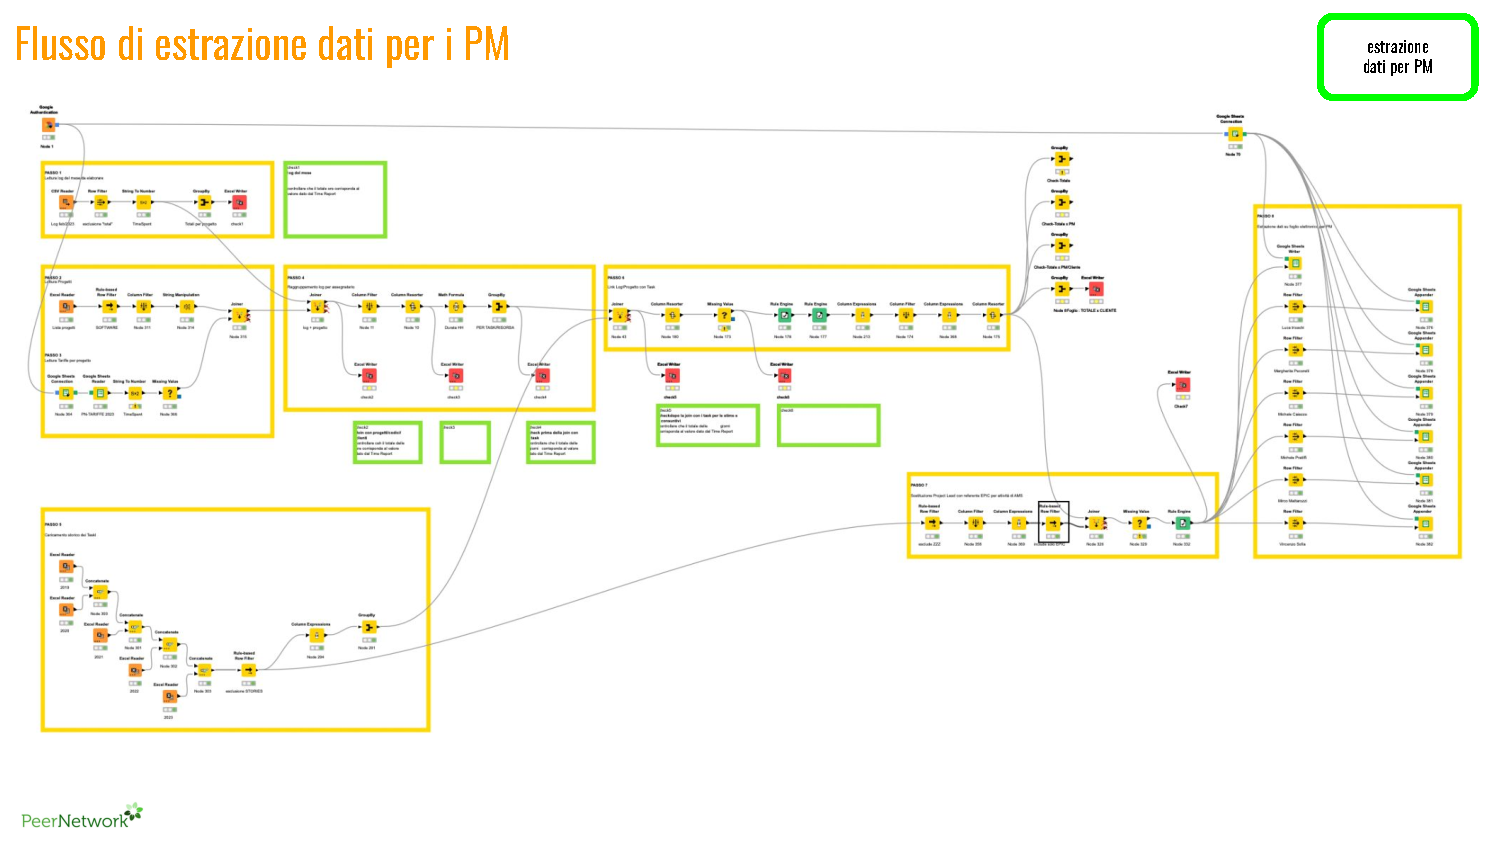
\includegraphics[width=\linewidth]{figures/FatturazioneKnime.pdf}
    \caption{Struttura su Knime riguardante una parte del processo di fatturazione, cioè l’estrazione di dati per i project manager}
    \label{fig:fatturazione-knime}
\end{figure}

Questo processo risultava troppo dispendioso in termini di tempo ed era basato su numerosi passaggi manuali. Per affrontare queste criticità, a gennaio 2024
è stato avviato il progetto interno \ac{PAM}, partendo con l’obiettivo di automatizzare gran parte del processo di fatturazione.
Le attività e il loro ordine di esecuzione sono schematizzate nella \Cref{fig:fatturazione}.

A partire da ottobre 2024, è stata resa disponibile la prima versione del sistema, che consente di completare l’intero flusso dal passaggio “estrazione dati
per PM” alla “generazione dei rapportini,” in poche ore anziché nelle circa due settimane precedentemente necessarie. L’utilizzo dei fogli elettronici da creare,
modificare o importare è stato completamente eliminato: l’intero processo è ora gestito dal gestionale, con l’utente che interagisce direttamente tramite un’unica
interfaccia grafica. L’automazione della fase di estrazione dati è stata resa possibile grazie all’integrazione con Jira\footnote{https://www.atlassian.com/software/jira},
uno strumento per la gestione e il monitoraggio dei progetti che consente ai dipendenti di registrare le ore lavorate su ciascun progetto.

\begin{figure}
    \centering
    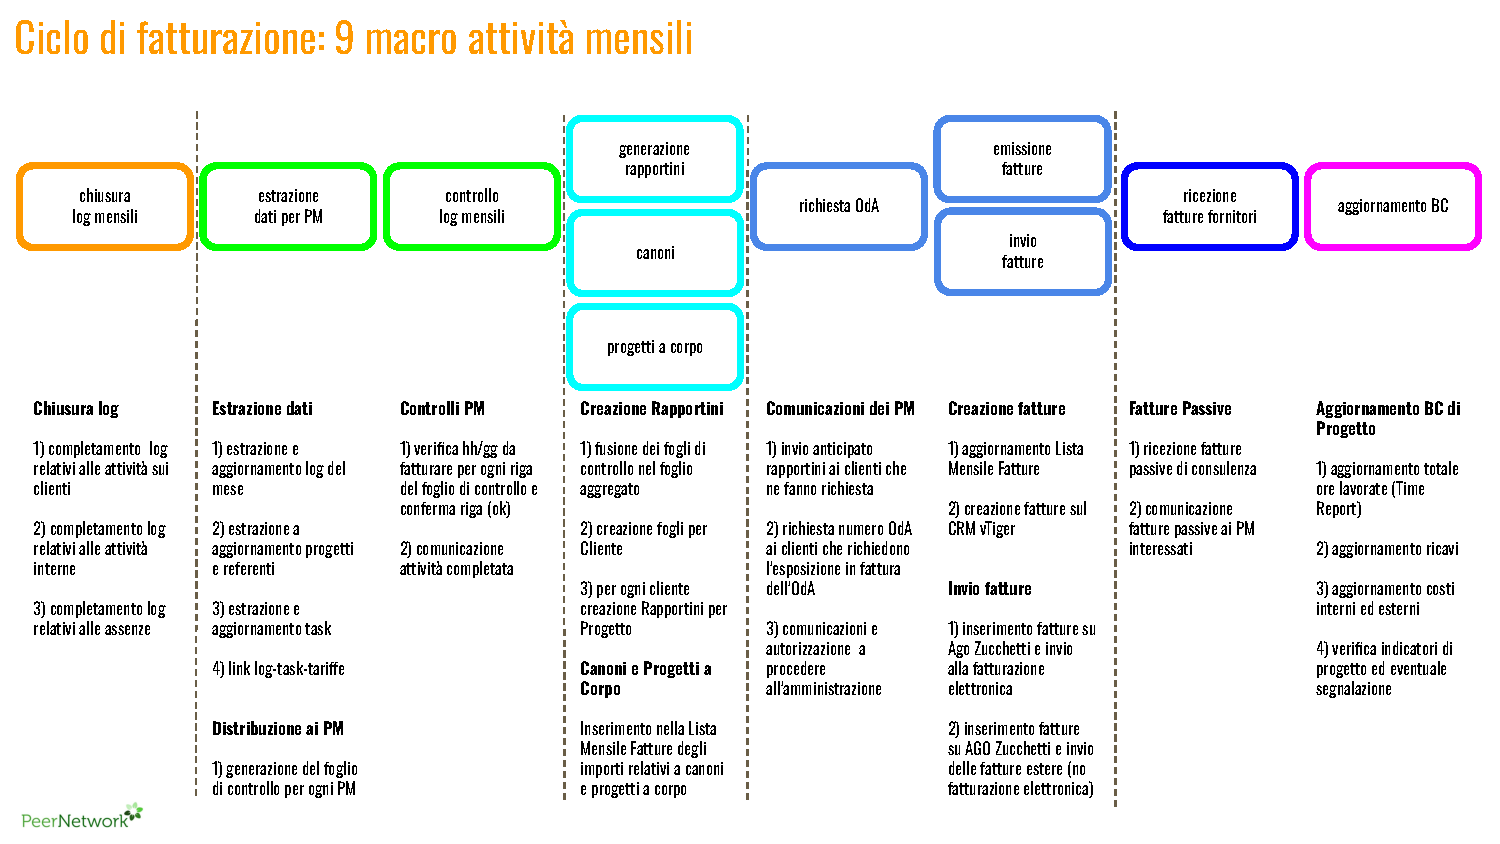
\includegraphics[width=\linewidth]{figures/fasiFatturazionePN.pdf}
    \caption{Attività presenti nel processo di fatturazione di \textit{Peer Network}}
    \label{fig:fatturazione}
\end{figure}

Le nuove funzionalità in fase di sviluppo, approfondite nel Capitolo \ref{chap:Results}, riguardano l’area dell’applicativo \ac{PAM} denominata \textbf{Progetti}, che verrà
utilizzata dalla direzione, dall’amministrazione e dai project manager. Questa sezione è pensata per centralizzare il controllo dei progetti, rendendo disponibili
informazioni generali, composizione dei team, tariffe orarie applicabili in base ai ruoli, situazione economica complessiva e dettagliata per mese, oltre alla
possibilità di consultare tutte le prefatture emesse.

Queste funzionalità semplificheranno notevolmente il lavoro degli utilizzatori, offrendo un unico punto di accesso per monitorare tutte le informazioni e mantenere
sotto controllo l’andamento dei progetti. Inoltre, la nuova gestione economica, sia generale che dettagliata, eliminerà la necessità di utilizzare i fogli elettronici
attualmente impiegati. Al momento, per ogni progetto viene creato un file separato per ogni anno solare, che deve essere aggiornato manualmente (come ultima fase del
processo di fatturazione nella \Cref{fig:fatturazione}) con i dati relativi a costi e ricavi effettivi, ricavi previsti per i mesi successivi e margini. Con la nuova area
Progetti, queste operazioni saranno automatizzate e integrate direttamente nell’applicativo.